\chapter{Ejemplo \emph{Euler-Lagrange} con Fricción}
\vspace{0.5cm}


\begin{adjustwidth}{50pt}{50pt}
\begin{ejemplo}
	En esta ocasión, vamos a ver la aplicación de las ecuaciones de \emph{Euler-Lagrange} a  un ejemplo de un sistema físico con rozamiento (proporcional a la velocidad), para encontrar las ecuaciones del movimiento.
\end{ejemplo}
\end{adjustwidth}

\vspace{0.5cm}

\section{Ecuaciones de \emph{Euler-Lagrange} con fricción}

\begin{tikzpicture}
	\fill [left color=red!50, right color=teal!50] (0,0) rectangle (6.5,.1);
	\fill [left color=teal!50, right color=blue!50] (6.5,0) rectangle (11.5,.1);
	\end{tikzpicture}

\vspace{1cm}



Vimos, en capítulo \ref{CapEEL}, las ecuaciones de Euler-Lagrange,

\begin{equation}
\boxed{ \ 
\dv{t} \left( \pdv{T}{\dot q} \right) \ - \ \pdv{T}{q} \ = \ Q \ = \ \overrightarrow F \cdot \pdv{\vec r}{q}	
\ }
\tag{\ref{T2PDD7}}
\end{equation}



Si consideramos que, además de fuerzas conservativas también va a haber fricción, $\ F=F^{Cons}+F^{Fric} \, , \ $ en $\ Q \ $ habrá dos términos: 

--- el correspondiente a las fuerzas conservativas, al provenir del gradiente de un potencial $\ V \ $escalar pasa a la izquierda y, junto con la energía cinética $\ T \ $ forman el lagrangiano $ \ L \ $ de las ecuaciones de Euler-Lagrange para el caso conservativo 

\begin{equation}
\boxed{
\dv{t} \left[ \pdv{ L }{\dot q} \right] \ - \ \pdv{L}{q} \ = \ 0	
\ } 
\tag{\ref{T2EEL1C}}
\end{equation}

--- el término de las fuerzas de fricción se queda en el miembro de la derecha y las \textbf{ecuaciones de Euler-Lagrange ante fuerzas conservativas y de  fricción} toman el siguiente aspecto:

\vspace{0.5cm}

\begin{large}
\begin{myblock}{\begin{normalsize}Ecuaciones de Euler-Lagrange ante fuerzas conservativas y de  fricción\end{normalsize}}
\begin{equation}
\label{T4EEF1}
\boldsymbol{ \
\dv{t} \left[ \pdv{ L }{\dot q} \right] \ - \ \pdv{L}{q} \ = \ Q_j^{Fric} \ = \ \sum_{i=1}^N \overrightarrow F_i^{Fric} \cdot \pdv{\overrightarrow r_i}{q_j}	
\ } 
\end{equation}	
\end{myblock}
\end{large}

\vspace{1cm}
\subsection{Ejemplo \emph{Euler-Lagrange} con fricción - 1}
\label{T4SecELF}
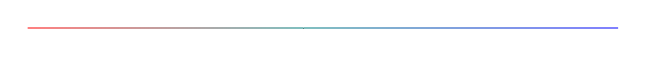
\begin{tikzpicture}
	\fill [left color=red!50, right color=teal!50] (0,0) rectangle (3.5,.01);
	\fill [left color=teal!50, right color=blue!50] (3.5,0) rectangle (7.5,.01);
	\end{tikzpicture}
\vspace{0.5cm}


\begin{example}
.	Una partícula de masa $M$ se encuentra en reposo en un punto sobre el eje $X$ (basta con suponer $M=\infty$). De ella cuelga una segunda partícula de masa $m$ suspendida de una barra rígida de masa despreciable y longitud $b$ a la que se la separa un ángulo $\theta$ de la vertical y se la deja oscilar libremente, pero se encuentra sometida a una fuerza de rozamiento $F$ proporcional a la velocidad. 	
	
	\vspace{2mm} Encontrar las ecuaciones del movimiento.

	\begin{figure}[H]
		\centering
		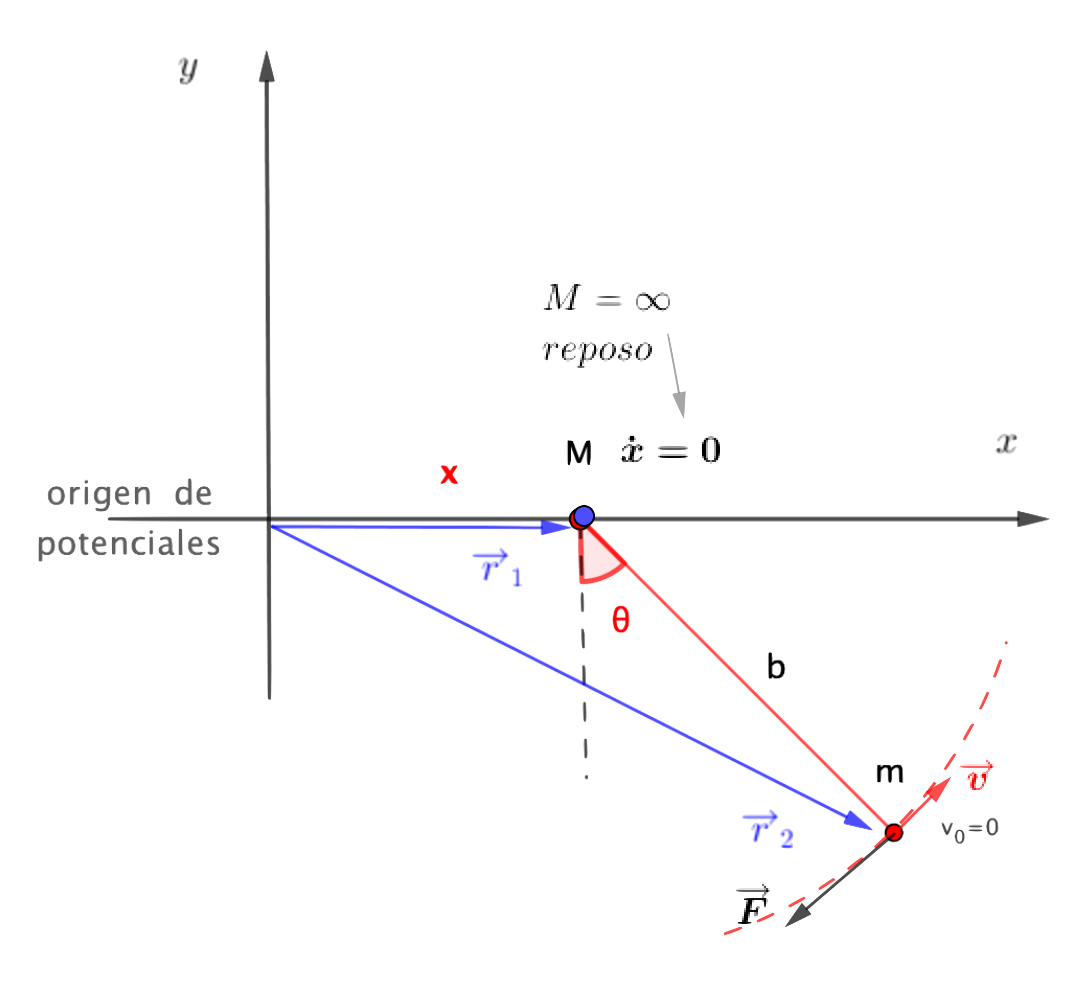
\includegraphics[width=.5\textwidth]{imagenes/img04-01.png}
		\end{figure}	
\end{example}

El ejemplo es el mismo que en el tema anterior (sección \ref{T3ejem}), por lo que el lagangiano será el mismo, pero teniendo en cuenta que la partícula de masa $M$ permanece en reposo, $\boldsymbol{\dot x=0}$,  particularizando ese resultado:

%\begin{small}
\begin{equation}
\tag{\ref{T3lagran}} 
 L=T-V=  
\cancelto{0}{ \dfrac 1 2 \ (M+m)\ \dot x^2 } + 
 \dfrac 1 2 \ m \ b^2 \ \dot \theta^2 +
 \cancelto{0}{ m \ b \ \dot \theta \ \dot x \cos \theta }+
 m\ g \ b \cos \theta 
\end{equation}
%\end{small}

El lagrangiano, en este caso, es:

\begin{equation}
\label{T4lagran-ejem1}
\boldsymbol{ 
 L\ = \ T-V \ = \  \dfrac 1 2 \ m \ b^2 \ \dot \theta^2  \ + \  m\ g \ b \cos \theta 
 }
\end{equation}

La fuerza de fricción (opuesta al movimiento) a la que se encuentra sometida $m$ es proporcional a la velocidad a la que ésta se mueve: $\ \overrightarrow F = - k \ \overrightarrow v$, es lo típico en el caso de movimiento es el seno de fluidos.

Calculamos la \emph{fuerza de fricción generalizada}, $Q^F$. Ahora solo tenemos una \emph{coordenada generalizada}, $\theta$.
$\quad \boldsymbol{ \displaystyle Q^F \ = \ \overrightarrow F \cdot \pdv{\overrightarrow r}{\theta} }$

Usando resultados que ya obtuvimos en el tema \ref{capejemEE}, en la sección \ref{T3ejem}, el vector de posición de las partícula $m$ es:

$\overrightarrow r = \overrightarrow r_2=\overrightarrow r_1+\overrightarrow b= (x,0)+(b\sin \theta,-b \cos \theta)=(x+b\sin \theta,-b \cos \theta)$

Derivando, $\quad \displaystyle \pdv{\overrightarrow r}{\theta}=b(\cos \theta, \sin \theta)$

Por lo que, $\quad \displaystyle Q^F=-K \overrightarrow v \cdot b (\cos \theta, \sin \theta)$

Veamos quién es $\overrightarrow v\, , \qquad \displaystyle \overrightarrow v=\dv{\overrightarrow r}{t}=(b \cos \theta \ \dot \theta, b \sin \theta \ \dot \theta)=b\ \dot \theta \ (\cos \theta, \sin \theta)$

Luego: $\quad \boldsymbol{ Q^F}=-kb\ \dot \theta \cdot b \ (\cos \theta, \sin \theta) =\boldsymbol{ -k\ b^2 \ \dot \theta }$

Llevando este resultado a las ecuaciones de Euler-Lagrange con fricción, ec \ref{T4EEF1}, y teniendo en cuenta cual es nuestro lagrangiano (ec. \ref{T4lagran-ejem1}),

$\begin{cases}
\ \ \displaystyle \dv{t} \left[ \pdv{L}{\dot \theta} \right] = \dv{t} [mb^2 \dot \theta]= m\ b^2 \ \ddot \theta 
\\ \\
\ \ \displaystyle \pdv{L}{\theta}=-mgb \sin \theta	
\end{cases} \quad \Rightarrow \quad m \ b^2\ \ddot \theta \ + \ m\ g\ b \ \sin \theta \ =\  -k\ b^2\ \dot \theta$

Pasando todo a la izquierda y dividiendo por $mb^2$,

\begin{equation}
\label{T4ecmonejem1}
\subrayado{ \ \boxed{ \ 	
\ddot \theta \ + \ \dfrac k m \ \dot \theta \ + \ \dfrac g b \ \sin \theta \ = \ 0 
\ } \ }
\end{equation}

Ecuaciones del movimiento. La dificultad para la resolución de esta ecuación diferencial estriba en la presencia del $\sin \theta$, pero podemos utilizar la \textbf{aproximación típica de ángulos pequeños}, $\ \ \boldsymbol{\theta << 1 \ \to \ \sin \theta \approx \theta}$. Con esto,

\begin{equation}
\label{T4ecmonejem1aprox}
\subrayado{ \ \boxed{ \ 	
\ddot \theta \ + \ \dfrac k m \ \dot \theta \ + \ \dfrac g b \  \theta \ = \ 0 
\ } \ }
\end{equation}

que es una EDO 2$^o$ orden lineal con coeficientes constantes homogénea, se puede resolver analíticamente. El resultado, ya conocido, es una oscilación que se va amortiguando con el tiempo.\footnote{ver al final del capítulo}

\begin{figure}[H]
		\centering
		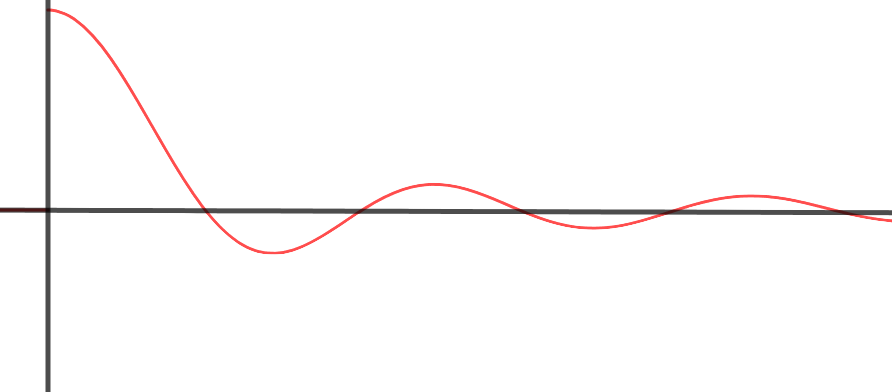
\includegraphics[width=.45\textwidth]{imagenes/img04-02.png}
		\end{figure}


\vspace{0.5cm}
\subsection{Ejemplo \emph{Euler-Lagrange} con fricción - 2}
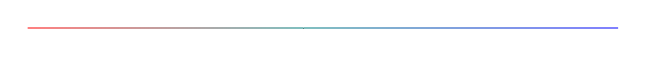
\begin{tikzpicture}
	\fill [left color=red!50, right color=teal!50] (0,0) rectangle (3.5,.01);
	\fill [left color=teal!50, right color=blue!50] (3.5,0) rectangle (7.5,.01);
	\end{tikzpicture}
%\vspace{0.5cm}

Supongamos ahora que $M$ también se puede mover y que también está sometida a una fuerza de fricción.

\vspace{0.5cm}
\begin{example}

\begin{multicols}{2}

	Una partícula de masa $M$ se mueve con rozamiento (proporcional a la velocidad) sobre el eje horizontal $X$. De ella cuelga una segunda partícula de masa $m$ suspendida de una barra rígida de masa despreciable y longitud $b$ a la que se la separa un ángulo $\theta$ de la vertical y se la deja oscilar pero también está sometida a un rozamiento proporcional a la velocidad con s¡que se mueve. 	
	
	\vspace{2mm} Encontrar las ecuaciones del movimiento.

	\begin{figure}[H]
		\centering
		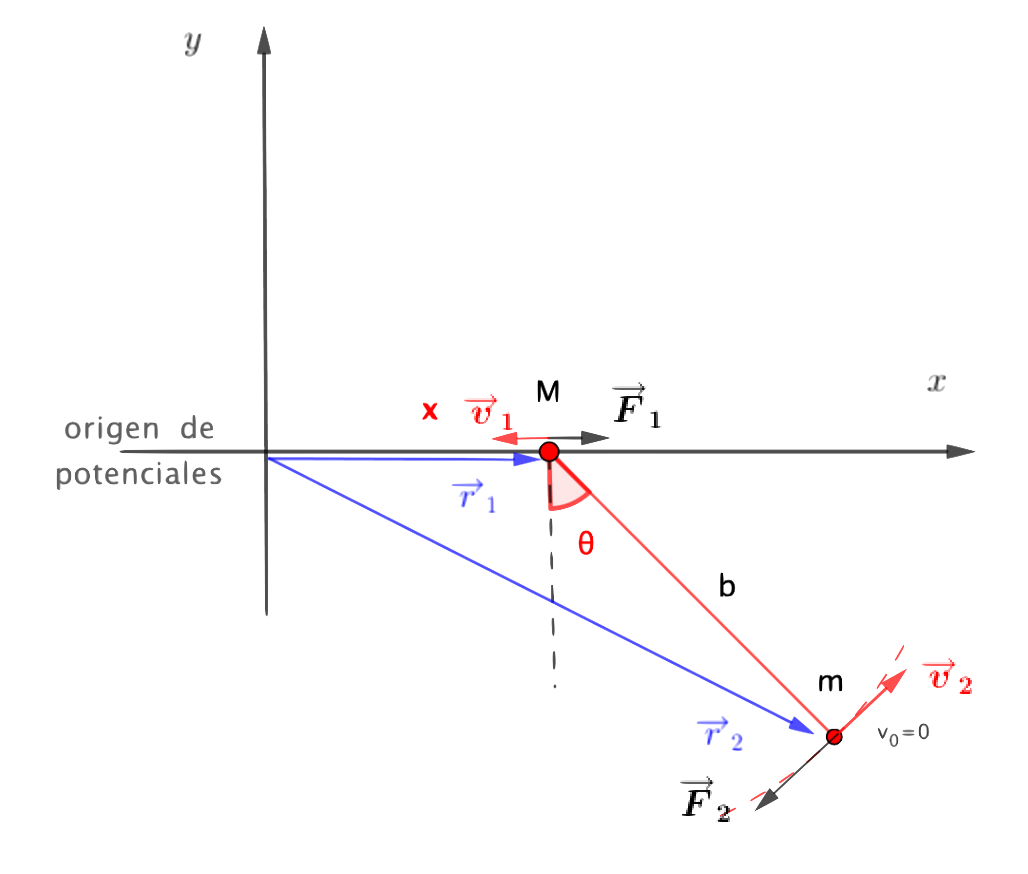
\includegraphics[width=.5\textwidth]{imagenes/img04-03.png}
		\end{figure}
\end{multicols}	
\end{example}

\vspace{0.5 cm}
\rule{200pt}{0.1pt}

Recuperamos los resultados obtenidos en el ejemplo del tema \ref{capejemEE}, en la sección \ref{T3ejem}, que siguen siendo válidos:

$ 
 L=T-V=  
 \dfrac 1 2 \ (M+m)\ \dot x^2  + 
 \dfrac 1 2 \ m \ b^2 \ \dot \theta^2 +
 m \ b \ \dot \theta \ \dot x \cos \theta +
 m\ g \ b \cos \theta 
$

$\begin{cases}
\ \overrightarrow r_1= (x,0) \\
\ \overrightarrow r_2=(x+b\sin \theta, -b\cos \theta	
\end{cases};
\quad
\begin{cases}
\ \overrightarrow v_1=(\dot x, 0) \\
\ \overrightarrow v_2=(\dot x + b \dot \theta \cos \theta, b \dot \theta \sin \theta)	
\end{cases}$

\begin{flushright}
\rule{200pt}{0.1pt}	
\end{flushright}

Calculemos, para más tarde, las siguientes derivadas:

$\displaystyle \pdv{\overrightarrow r_1}{x}=(1,0)\, ; \qquad \pdv{\overrightarrow r_2}{x}=(1,0)$

$\displaystyle \pdv{\overrightarrow r_1}{\theta}=(0,0)\, ; \qquad \pdv{\overrightarrow r_2}{\theta}=(b\cos \theta, b \sin \theta))$

\vspace{0.5cm}
Ahora, al aplicar las ecuaciones de Euler-Lagrange al caso en que haya fricción (ec. \ref{T4EEF1}), el miembro de la izquierda es el mismo que en el ejemplo de la sección \ref{T3ejem} del tema \ref{capejemEE} y, en el miembro de la derecha, tenemos que calcular las fuerzas generalizadas $Q^F_j$ debidas a las fuerzas de fricción $F_1$ que actúa sobre la partícula de masa $M$ y $F_2$ sobre $m$:

$\overrightarrow F_1 \ = \ - k_1\ \overrightarrow v_1 \, ; \qquad 
\overrightarrow F_2 \ = \ - k_2 \ \overrightarrow v_2$

Como hay dos coordenadas generalizadas, $q_1=\dot x \text{ y } q_2=\theta$, tendremos dos fuerzas generalizadas asociadas, $Q_x \text{ y } Q_{\theta}$

$\boxed{ \Rightarrow \  \ \boldsymbol {Q_x} \, : \ }$
$\qquad$
$Q_x=\displaystyle \sum_{i=1}^{2} \overrightarrow F_i \cdot \pdv{\overrightarrow r_i}{x} = 
\overrightarrow F_1 \cdot \pdv{\overrightarrow r_1}{x}+
\overrightarrow F_2 \cdot \pdv{\overrightarrow r_2}{x}$

$Q_x=-k_1\overrightarrow v_1 \cdot (1,0) - k_2 \overrightarrow v_2 (1,0)=-(k_1\overrightarrow v_1+k_2 \overrightarrow v_2) \cdot (1,0)=$

$Q_x=-[k_1(\dot x,0)+k_2(\dot x+b\dot \theta \cos \theta, b \dot \theta \sin \theta)]\cdot (1,0)=-k_1 \dot x - k_2(\dot x+b\dot \theta \cos \theta)$


\begin{equation}
Q_x \ = \ -(k_1+k_2) \ \dot x \ - \  k_2 \ b \ \dot \theta \cos \theta	
\end{equation}



$\boxed{\Rightarrow \  \ \boldsymbol {Q_{\theta}} \, : \ }$
$\qquad$
$Q_{\theta}=\displaystyle \sum_{i=1}^{2} \overrightarrow F_i \cdot \pdv{\overrightarrow r_i}{{\theta}} = 
\overrightarrow F_1 \cdot \pdv{\overrightarrow r_1}{{\theta}}+
\overrightarrow F_2 \cdot \pdv{\overrightarrow r_2}{{\theta}}$

$Q_\theta= \cancel{ -k_1 \overrightarrow v_1 \cdot (0,0)} - k_2 \overrightarrow v_2 \cdot b(\cos \theta, \sin \theta)$

$Q_\theta=-k_2(\dot x + b \dot \theta \cos \theta, b \dot \theta \sin \theta) \cdot b (\cos \theta, \sin \theta)$

$Q_\theta=-k_2b[\dot x \cos \theta + b \dot \theta \cos^2 \theta+b \dot \theta \sin^2 \theta]=-k_2 b [\dot x + b \dot \theta]$

\begin{equation}
Q_\theta \ = \ -k_2\ b \ \dot x \ \cos \theta - k_2 \ b^2 \ \dot \theta	
\end{equation}

Recuperando la parte conservativa de las ecuaciones de. movimiento encontradas en el ejemplo de la sección \ref{T3ejem} del tema \ref{capejemEE} para la coordenada generalizada $\boldsymbol x$ :

$(M+m)\ \ddot x + m\ b [\ddot \theta \cos \theta -\dot \theta^2 \sin \theta]\ \textcolor{gris}{ \ (= \ 0 \text{ antes, ahora}  ) \ } = \ Q_x\, , \  $ luego 

\begin{equation}
\boldsymbol{
	(M+m)\ \ddot x + m\ b \ [\ \ddot \theta \cos \theta -\dot \theta^2 \sin \theta \ ] \ = \ \ -(k_1+k_2) \ \dot x \ - \  k_2 \ b \ \dot \theta \cos \theta	
}
\end{equation}

Procediendo del mismo modo para $\boldsymbol \theta$

$m\ b^2 \ \ddot \theta \ + \ m \ b \ddot x \ \cos \theta \ + \ m\ g \ b \sin \theta \ \textcolor{gris}{ \ (= \ 0 \text{ antes, ahora}  ) \ } =\ Q_\theta$ 

\begin{equation}
\boldsymbol{
m\ b^2 \ \ddot \theta \ + \ m \ b \ddot x \ \cos \theta \ + \ m\ g \ b \sin \theta \ = \ -k_2\ b \ \dot x \ \cos \theta - k_2 \ b^2 \ \dot \theta	
}
\end{equation}

Resumiendo,

\begin{myalertblock}{Ecuaciones del movimiento con rozamiento}
\begin{equation}
\begin{cases}
\ \ \boldsymbol{
	(M+m)\ \ddot x + m\ b \ [\ \ddot \theta \cos \theta -\dot \theta^2 \sin \theta \ ] \ = \ \ -(k_1+k_2) \ \dot x \ - \  k_2 \ b \ \dot \theta \cos \theta	
}
\\ \\ 	
\ \ \boldsymbol{
m\ b^2 \ \ddot \theta \ + \ m \ b \ddot x \ \cos \theta \ + \ m\ g \ b \sin \theta \ = \ -k_2\ b \ \dot x \ \cos \theta - k_2 \ b^2 \ \dot \theta	
}
\end{cases}
\end{equation}
\end{myalertblock}


La resolución de etas ecuaciones requiere de una simulación numérica.


\vspace{1cm}
\begin{center}
	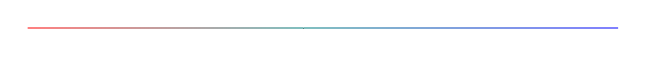
\begin{tikzpicture}
	\fill [left color=red!50, right color=teal!50] (0,0) rectangle (3.5,.01);
	\fill [left color=teal!50, right color=blue!50] (3.5,0) rectangle (7.5,.01);
	\end{tikzpicture}
\end{center}
\vspace{1cm}




\begin{myexampleblock} {Oscilaciones amortiguadas}

\begin{small}

\vspace{2mm}En la naturaleza, los movimientos oscilatorios no existen. Van perdiendo amplitud paulatinamente hasta que se detienen debido a las fuerzas de rozamiento.

\vspace{2mm}Resolvamos la ecuación diferencial de segundo orden lineal y homogénea obtenida en la sección \ref{T4SecELF}, ec. \ref{T4ecmonejem1}:

 $$\boldsymbol{\ \displaystyle m \ \ddot \theta \ + \ k \ \dot \theta \ + \ k  \theta\ = \ 0 \ }$$


\vspace{2mm} La ecuación característica asociada a esta EDO es: 

\vspace{2mm}
$\ mp^2+kp+g=0 \to p=
\dfrac{-k\pm\sqrt{k^2-4mg}}{2m}
-\dfrac {k}{2m} \pm \left[ \left( \dfrac {k}{2m} \right)^2 - \left( \dfrac g m \right) \right]^{1/2}$

\vspace{2mm} Llamamos $\gamma=\dfrac {b}{2m}$, \emph{coeficiente de amortiguamiento} y $\omega^2=\dfrac{k}{m}$, que en el caso del oscilador armónico es la frecuencia angular.

\vspace{2mm} Las soluciones de la ecuación característica son, ahora, $p=-\gamma \pm \sqrt{\gamma^2-\omega^2}$

\vspace{2mm} Vamos a estudiar tres casos:

\begin{itemize}
\item $\gamma < \omega \qquad$ (raíces $p$ imaginarias - \emph{infraamortiguado})

$(\gamma^2-\omega^2)^{1/2}=i\ (\omega^2-\gamma^2)^{1/2}=\pm \ i \ \omega_1 \to p=-\gamma \pm \ i \ \omega_1$

\begin{multicols}{2}
La solución general es estos casos es: $\quad \theta=Ae^{-\gamma t}\cos(\omega_1t+\alpha)$

$A e^{-\gamma t}$ es la amplitud instantánea. Se trata del tipo de movimiento del péndulo simple.
\begin{figure}[H]
		\centering
		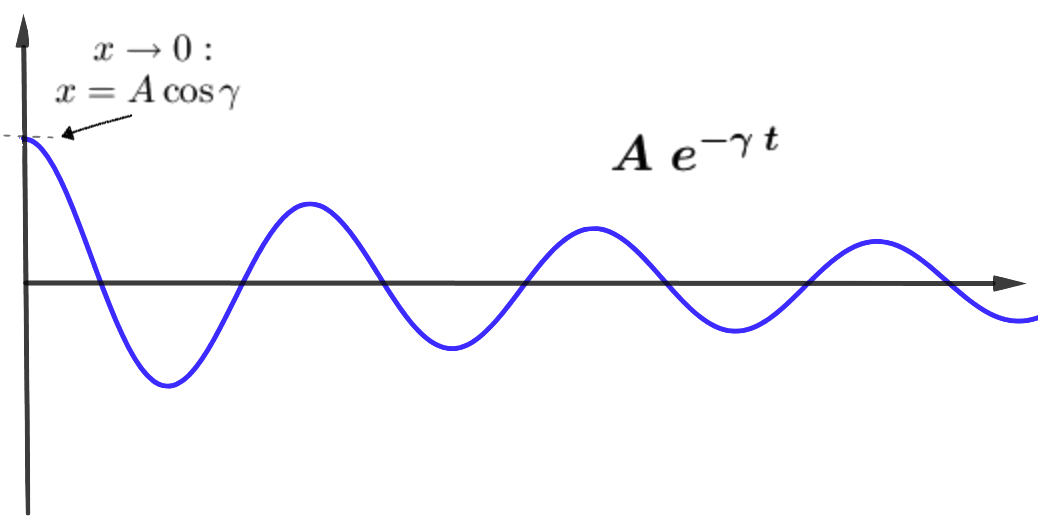
\includegraphics[width=.45\textwidth]{imagenes/img04-04.png}
	\end{figure}
\end{multicols}

\item $\gamma > \omega \qquad$ (raíces $p$ reales y distintas - \emph{sobreamortiguado})

$p_1=-\gamma + (\gamma^2-\omega^2)^{1/2}=-\gamma_1; \quad
p_2=-\gamma - (\gamma^2-\omega^2)^{1/2}=-\gamma_2 $

La solución más general es: $\theta=Ae^{-\gamma_1 t}+Be^{-\gamma_2 t}$

\begin{multicols}{2}
Exponenciales decrecientes; en este caso, la amplitud decae más rápidamente que en el anterior.

Es el caso de un péndulo muy ligero oscilando sumergido en agua.
\begin{figure}[H]
		\centering
		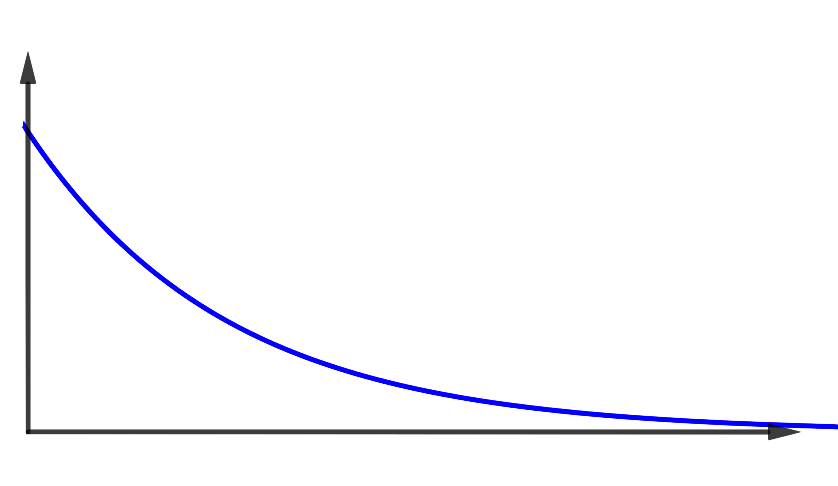
\includegraphics[width=.45\textwidth]{imagenes/img04-05.png}
	\end{figure}
\end{multicols}
\item $\gamma = \omega \qquad$	($p$ es una raíz real doble - \emph{amortiguamiento crítico})

$p=-\gamma  \to \theta=(A+Bt)e^{-\gamma t}$

\end{itemize}
\vspace{2mm}
\begin{multicols}{2}
 El amortiguamiento crítico proporciona la forma más rápida de aproximar a cero la amplitud de un oscilador amortiguado. Con menor amortiguamiento (subamortiguación) alcanza el cero más rápidamente, pero oscila alrededor de él. Con mas amortiguamiento (sobreamortiguación), el acercamiento a cero es más lento. La amortiguación crítica, ocurre cuando el coeficiente de amortiguación es igual a la frecuencia de resonancia sin amortiguación del oscilador.


\begin{figure}[H]
		\centering
		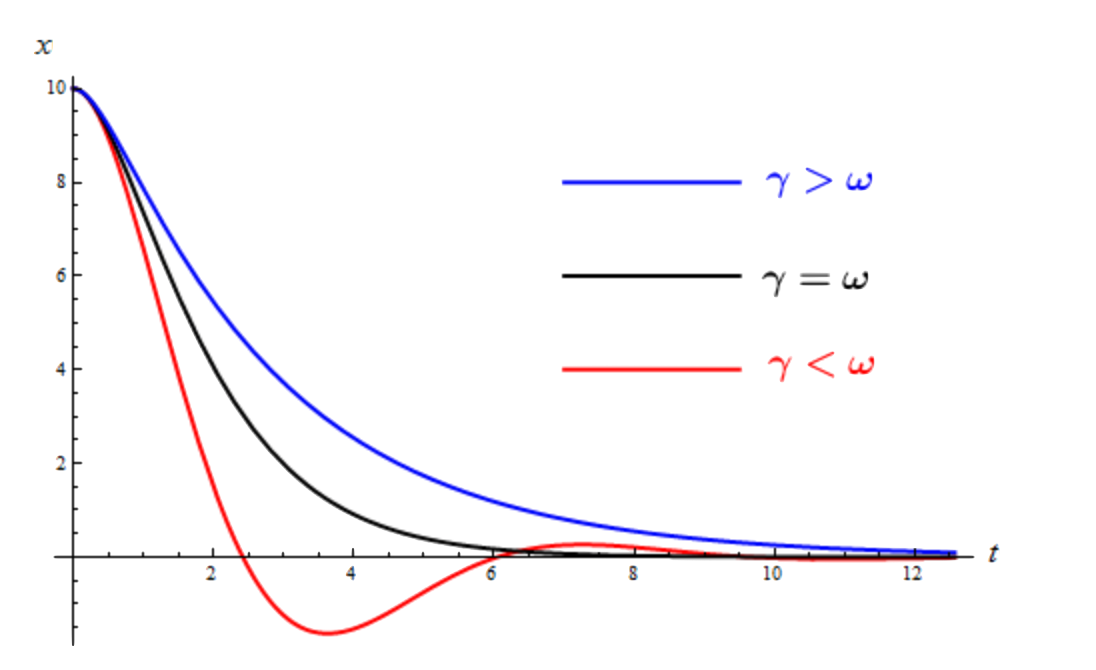
\includegraphics[width=.5\textwidth]{imagenes/img04-06.png}
	\end{figure}

\end{multicols}
\end{small}

\rule{300pt}{0.1pt}
\begin{flushright} \begin{footnotesize}
	\textcolor{gris}{`Fisica General', Ignacio Vallés, http://igvaori.github.io}
\end{footnotesize} \end{flushright}


\end{myexampleblock}

